\documentclass[a4paper]{article}
\usepackage[utf8]{inputenc}
\usepackage[L7x]{fontenc}
\usepackage[lithuanian]{babel}
\usepackage{lmodern}
\usepackage{graphicx}
\usepackage[top=2cm, bottom=2cm, left=1.5cm, right=1.5cm, footskip=1cm, a4paper]{geometry}
\usepackage{verbatim}
\usepackage{amsmath,amsfonts,amssymb,amsthm}
\usepackage{colortbl}
\usepackage{tcolorbox}
%\usepackage{indentfirst}
%\usepackage{framed}
%\usepackage{tikz}
\usepackage{xcolor}
%\usepackage[unicode]{hyperref}
%\usepackage{minted}
%\usepackage{cancel}
%\usepackage{framed}

\newcommand{\true}[1]{\cellcolor{green!80!black}{#1}}
\newcommand{\false}[1]{\cellcolor{red}{#1}}
\begin{document}
Pradėjome nuo 2015 metų testinės dalies įsivertinimo. \\
\\
%use \colorbox{green!80!black}{E} for overriding color
\begin{tabular}{|l|l|l|l|}
\hline
Uždavinys & Teisingas atsakymas & Elžbietos ats. & Sritis\\ \hline\hline
1. & C & D & \false{Funkcijos} \\ \hline
2. & 14 & 14 & \true{Funkcijos}\\ \hline
3. & 350 eur. & 350 eur. & \true{Reiškinių sudarymas}\\ \hline
4. & 10 & - & \false{Statistika}\\ \hline
5. & 8 val. & 2 val? & \false{Reiškinių sudarymas}\\ \hline
6. & -2013 ir -2014 & - & \false{Elementarūs algebriniai pertvarkymai}\\ \hline
7. & -1 & - & \false{Vektoriai}\\ \hline
8. & $60^o$ & - & \false{Geometrija}\\ \hline
9. & 120 & $9\times 8 \times 7$ & \false{Kombinatorika}\\ \hline
10. & $a-b$ & - & \false{Funkcijos}\\ \hline
11. & $[2; 3)$ & - & \false{Funkcijos}\\ \hline
12. & Ar norėtum dar pasibandyti? & - & \\ \hline
13. & $\begin{array}{l} \text{a)}\angle ABC = 40^o \\ \text{b)} \angle{AMB} = 100^o \end{array}$ & D & \false{Geometrija}\\ \hline
14. & $180$ & - & \false{Geometrija}\\ \hline
15. & $\begin{array}{l} \text{a)}(-\infty; -2)\text{ ir }(1; 6)\\ \text{b)} 1 \end{array}$ & D & \false{Išvestinės}\\ \hline
16. & a) $\overrightarrow{AC}$ b) 0& - & \false{Vektoriai}\\ \hline
17. & a) 10 b) 11,8 & - & \false{Trigonometrija} \\ \hline
\end{tabular}
\\
\\
Priminsiu, kad preliminarūs egzamino temų svoriai yra tokie:
\\
\\
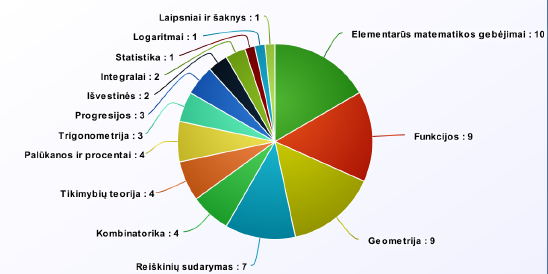
\includegraphics[width = 0.6\textwidth]{pasiskirstymas.png}

Netrukus paskutiniame stulpelyje patalpinsiu savo priskirtus sričių pavadinimus, įvardysiu gebėjimus arba turinio žinias, kurių reikia tose srityse pasistumti ir pridėsiu nuorodas į šaltinius. Taip pat pabandysiu surašyti įvairius kilusius klausimus ir atsakymus, kaip kas sprendžiama.
\section*{Klausimai}
\begin{enumerate}
\item Kaip išmokti atskirti funkcijų grafikus?
\item Kaip išmokti atlikti stebėjimus?
\item Kaip išmokti tokias sąvokas kaip mediana?
\item Kalbėjome apie kubą su dukart padidėjusia kraštine ir ritinio tūrio skaičiavimą. Kaip šiuos dalykus išmokti?
\item Kaip išmokti geometriją?
\item Kaip su kitomis temomis?
\end{enumerate}
\section*{Atsakymai}
\begin{enumerate}
\item Mokymasis turėtų susidėti iš kelių etapų: iš pradžių prisiminsime, kaip braižyti funkcijas, tada atliksime stebėjimus (kas keičiasi grafike, kai keičiasi argumento reikšmė), tada apibendriname visas pasitaikančias grafikų formas. 
\item Atsakymas labai platus; norint į jį rasti atsakymus reikės pasinagrinėti temą \textit{developmental stages}. Šiai temai aptarti skirsime laiko atskirai. 
\item Patariu pasikartoti visas savokas apie statistiką, tokias kaip moda, mediana, vidurkis. Jas išmokti nesunku, o išmokus šią temą galime uždaryti.
\item Reikėtų pradėti nuo tūrio sąvokos aiškinimosi. Atliksime išsamią tūrio vaizdinio analizę.
\item Su geometrija neskubėkime, nes man dar reikia susirinkti ir išanalizuoti praėjusių metų uždavinius, kad būtų galima aiškiau išskirstyti temas. Kol kas paliesime tik tūrį ir įbrėžtinius kampus.
\item Kitoms temoms (funkcijos, vektoriai, trigonometrija, šiek tiek kombinatorika) turiu parengęs ruošimosi planus.
\end{enumerate}
\end{document}